\section{Comparison---Systematic Generalization via Parallel Circuit}
\label{sec:comparison}
We have just shown that the vanilla transformer fails to achieve OOD generalization for composition, \textit{but is the vanilla transformer generally incapable of acquiring systematic implicit reasoning skills?} We show that for \textit{comparison}, a task where SoTA LLMs such as GPT-4 also struggle~\citep{allenzhu2023physics}, the vanilla transformer \textit{does} have the capability to acquire systematic generalization, again through grokking. On the surface, it seems that the comparison task is no different than the composition task---both require retrieving and reasoning over two pieces of facts. However, as it turns out through our analysis, \textit{the comparison task emits a ``parallel circuit'' that is learned by the transformer during grokking, which allows atomic facts to be stored and retrieved in the same region and enables systematicity to happen.}

\noindent\textbf{Setup.} The comparison task involves comparing the attribute values of entities. We assume there are $|\mathcal{E}|=1000$ entities, $|\mathcal{A}|=20$ attributes and $|\mathcal{V}|=20$ ordinal values for the attributes. Each attribute $a\in \mathcal{A}$ has a label space $\{a_<, a_=, a_>\}$, a set of relations specifying its comparative form. For example, an attribute \textit{age} would have $a_<, a_=, a_>$ to be \textit{younger, contemporary, older}, respectively.

The atomic facts are \textit{(entity, attribute, value)} triplets, where we assign a random value $v\in \mathcal{V}$ for each $(e, a) \in \mathcal{E}\times \mathcal{A}$. Again, we randomly partition the atomic facts into \ttsmall{atomic$_{\text{ID}}$} and \ttsmall{atomic$_{\text{OOD}}$} (\num{90}\%: \num{10}\%). The rules of comparison are: 
\begin{equation}
\label{eq:comparison}
    \begin{aligned}
    & \forall e_1,e_2\in \mathcal{E},\forall a\in \mathcal{A}, \forall v_1,v_2\in \mathcal{V},(e_1, a, v_1)\land(e_2, a, v_2)\land v_1 < v_2 \implies (a, e_1, e_2, a_<),\\
    & \forall e_1,e_2\in \mathcal{E},\forall a\in \mathcal{A}, \forall v_1,v_2\in \mathcal{V},(e_1, a, v_1)\land(e_2, a, v_2)\land v_1=v_2 \implies (a, e_1, e_2, a_=),\\
    & \forall e_1,e_2\in \mathcal{E},\forall a\in \mathcal{A}, \forall v_1,v_2\in \mathcal{V},(e_1, a, v_1)\land(e_2, a, v_2)\land v_1>v_2 \implies (a, e_1, e_2, a_>).\\
    \end{aligned}
\end{equation}
Take the attribute \textit{age} as an example, the first rule means if the \textit{age} of $e_1$ is \textit{smaller than} the \textit{age} of $e_2$, then we can infer ``In terms of \textit{age}, the relation between $e_1$ and $e_2$ is \textit{younger}''. Each entity/attribute/value/label is assigned a unique token, and training/testing is done by having the model predict the last token (attribute value for atomic facts; comparative relation for inferred facts).

\noindent\textbf{Results \& analysis}. Figure~\ref{fig:grokking}(right) shows the results for $\phi=7.2$, and we include more results in Appendix~\ref{app:comparison_phi}. It can be seen that 1) the model again acquires robust generalization only through grokking; 2) surprisingly, the model also achieves systematicity in generalization, different from the case of composition.

Analyzing the model's internals similarly as in \S\ref{grokkinganalysis} (details in Appendix~\ref{app:circuit}), we find the generalizing circuit for comparison illustrated in Figure~\ref{fig:circuit_comparison}(a). On a separate stream, the model prepares the label space $\{a_<, a_=, a_>\}$ from $a$ and stores it in $S[7,a]$. In the lower layers (\num{0}-\num{5}), the model retrieves the two atomic facts and stores the attribute values $v_1$ and $v_2$ at $S[5,e_1]$ and $S[5,e_2]$. Then, the upper layers (\num{5}-\num{8}) compare $v_1,v_2$ and fetch the label from $S[7,a]$ based on the comparison result. Importantly, there is a major difference compared with the circuit for composition: the two atomic facts are retrieved \textit{in parallel}, which suggests that the atomic facts are stored solely in the lower layers, without having separate copies across different regions as in the circuit for composition. This explains why systematicity could happen: OOD facts are now stored and accessed in the same way as ID facts. Tracking the changes in the model throughout grokking, we observe significantly strengthened causal connections from $S[7,a]$ and $S[5,e_1]$ to the final prediction (Figure~\ref{fig:circuit_comparison}(b)). We also find that throughout grokking, $S[7,a]$ always encodes the label space and $S[5,e_1], S[5,e_2]$ gradually encode the two attribute values (Figure~\ref{fig:circuit_comparison}(c)). This confirms that a similar transition from $C_{mem}$ to $C_{gen}$ happens during grokking.

\vspace{-5pt}
\begin{figure}[h]
\centering
\begin{subfigure}{0.36\textwidth}
    \centering
    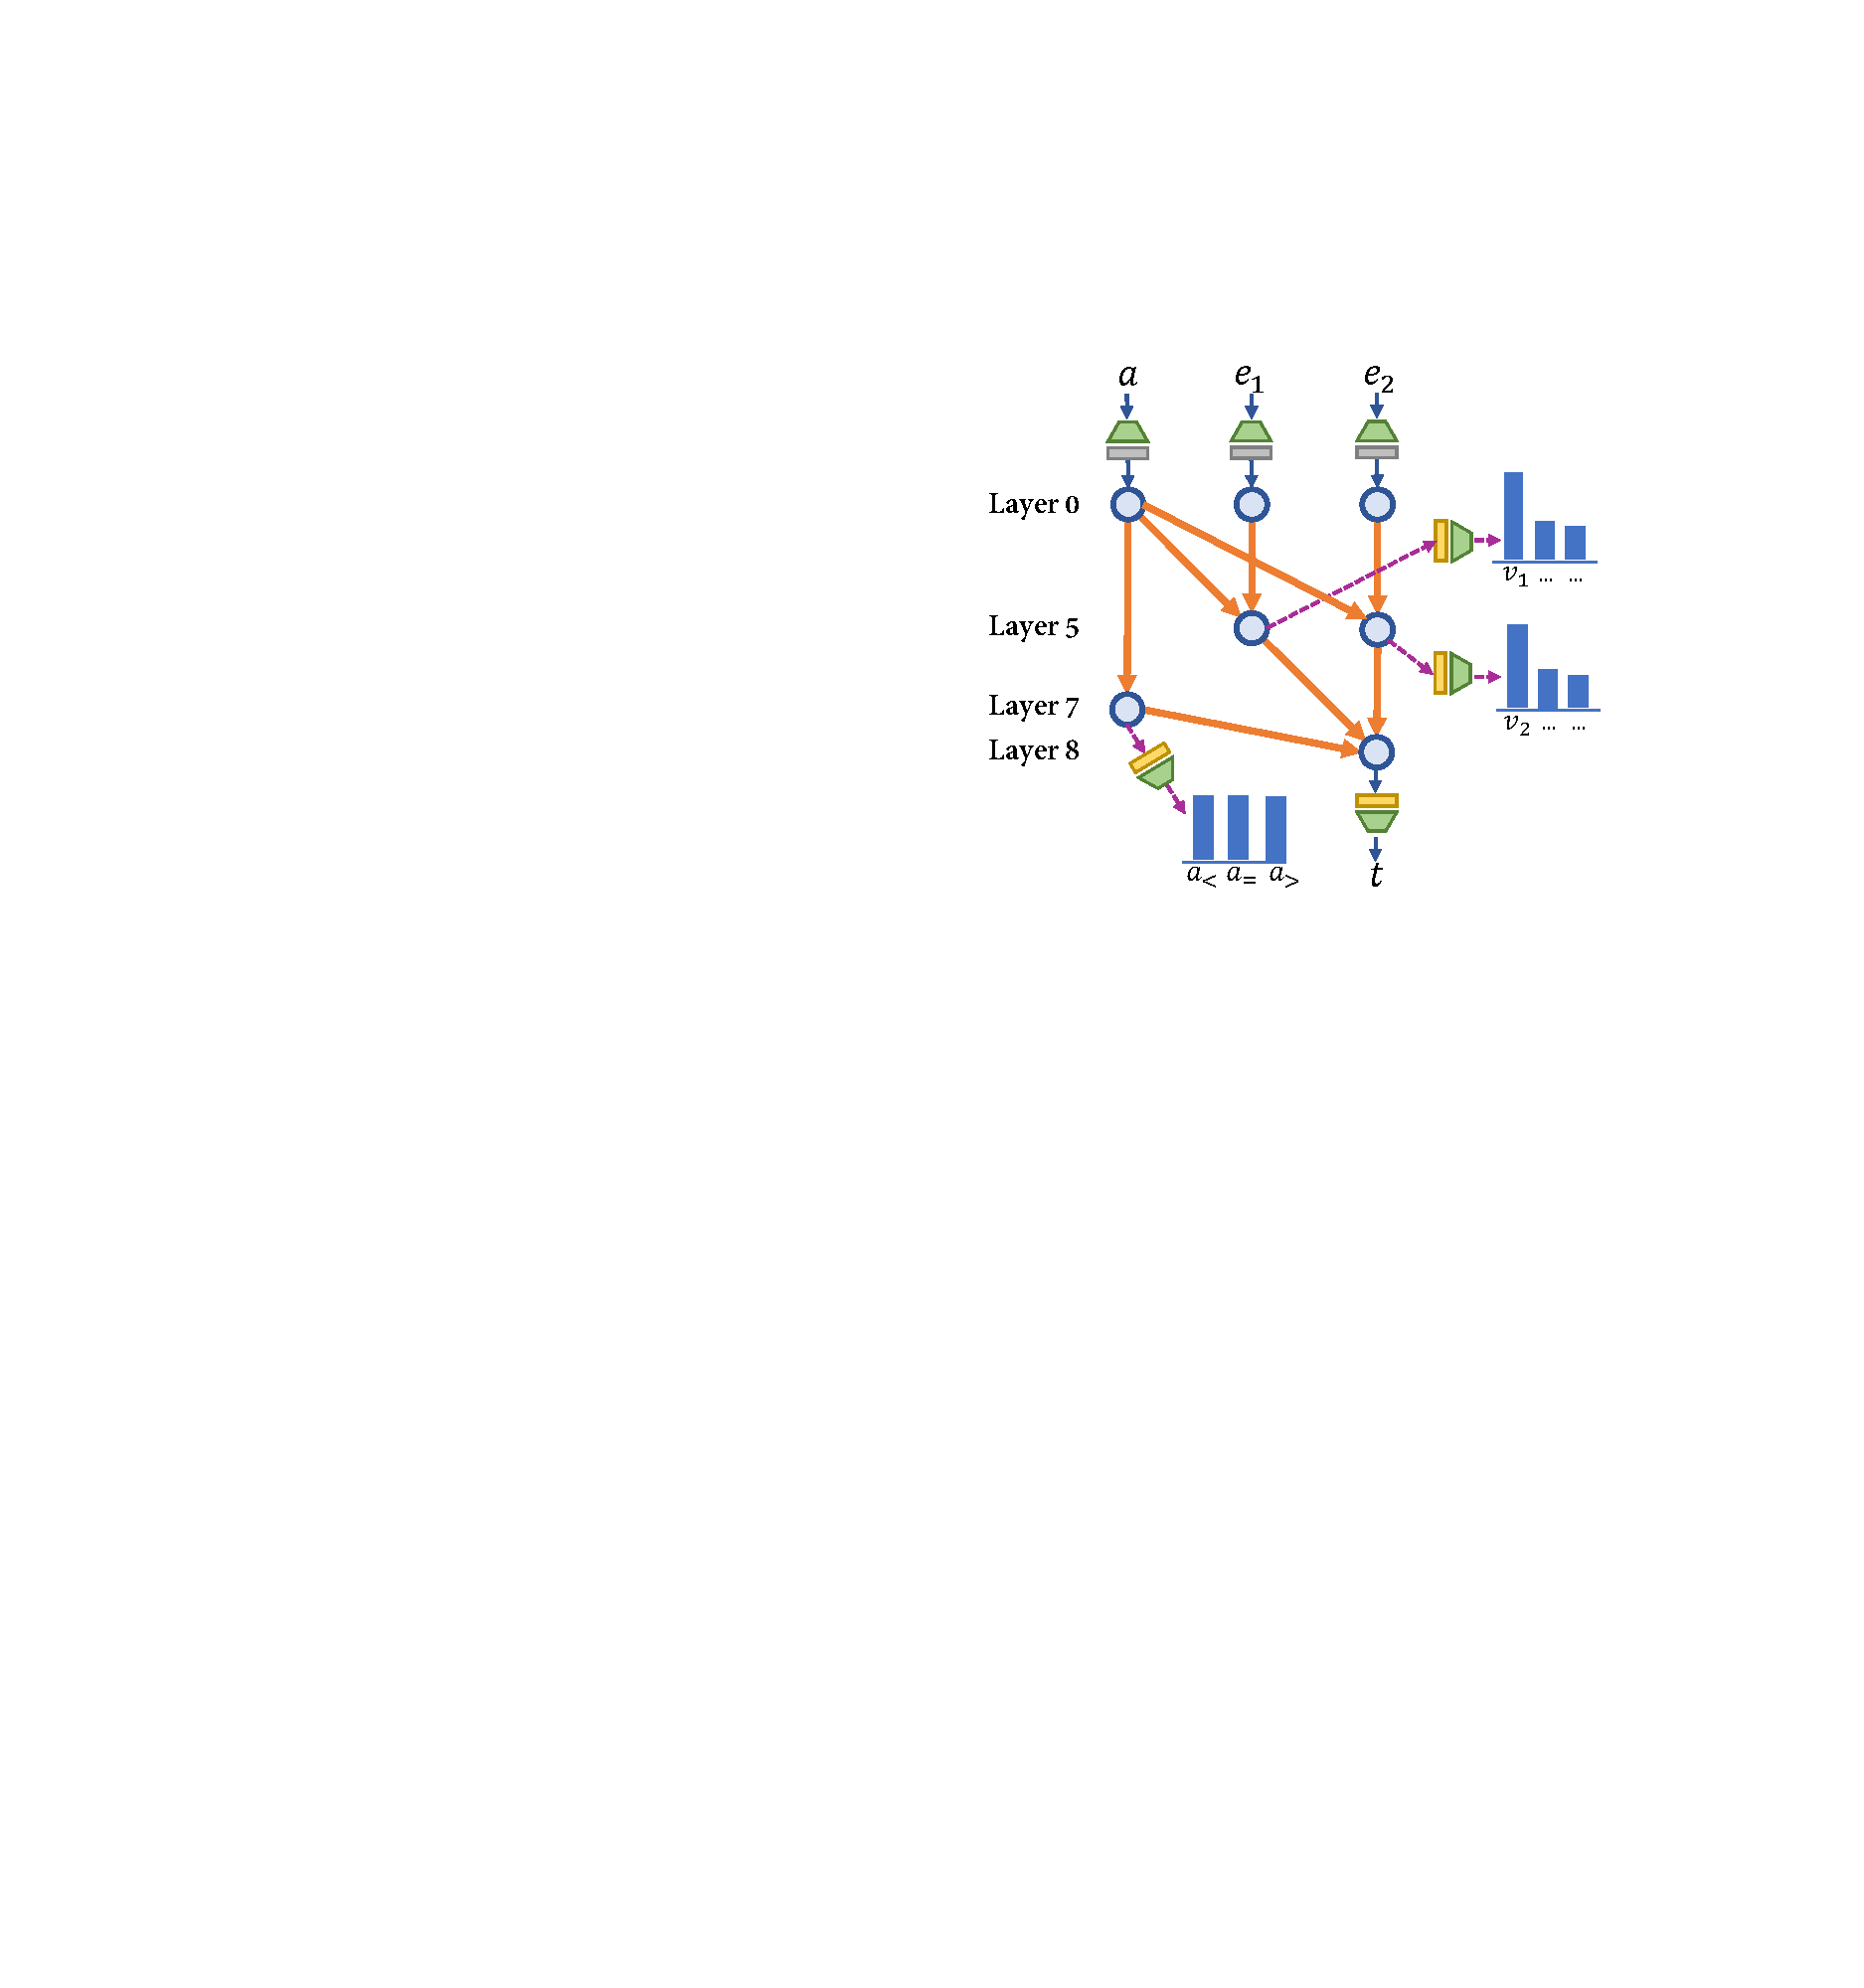
\includegraphics[width=\textwidth]{fig/circuit_comparison.pdf}
    \caption{}
\end{subfigure}
\begin{subfigure}{0.25\textwidth}
    \centering
    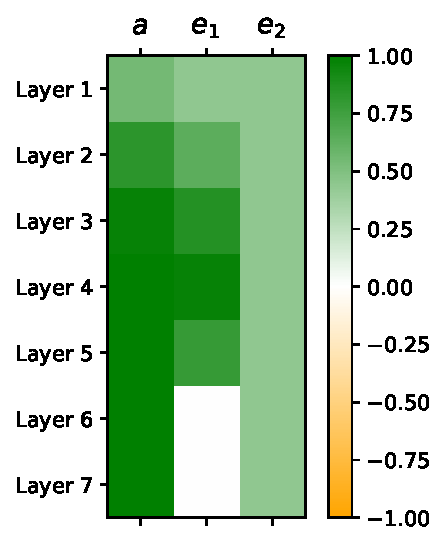
\includegraphics[width=\textwidth]{fig/causal_comparison_diff.pdf}
    \caption{}
\end{subfigure}
\begin{subfigure}{0.35\textwidth}
    \centering
    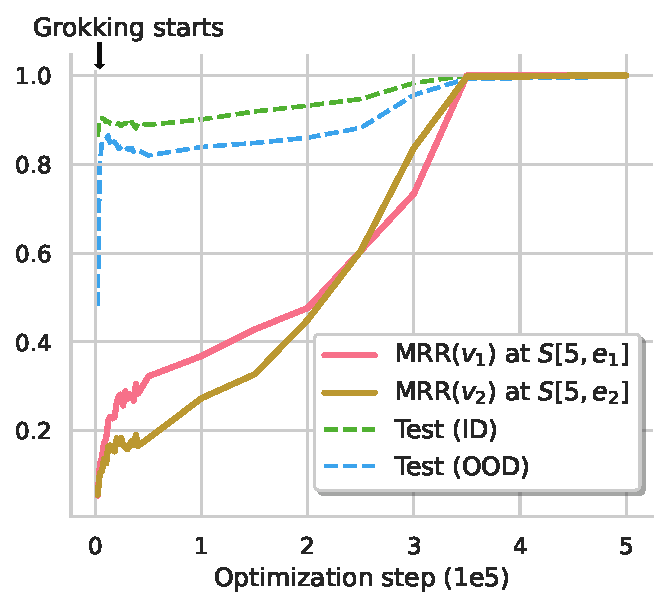
\includegraphics[width=\textwidth]{fig/MRR_comparison.pdf}
    \caption{}
\end{subfigure}
\caption{The (evolution of) generalizing circuit for comparison. (a) The generalizing circuit. (b) The \textit{change} in causal strengths during grokking, where the target is the prediction state. (c) Mean reciprocal rank (via logit lens) of the two attribute values ($v_1, v_2$) at $S[5,e_1]$ and $S[5,e_2]$.}
\label{fig:circuit_comparison}
\end{figure}

The findings here showcase transformer's ability to learn parallel solutions to seemingly sequential problems, akin to the findings in Liu et al.~\citep{liu2023transformers} where it is shown that transformers can learn ``shortcuts'' to automata. The difference in the acquired generalization across the two tasks that we study also emphasizes the need for \textit{controlled and mechanistic} study on understanding the transformer's reasoning before making general claims on its limitations.